\documentclass[a4paper,12pt]{article}

\usepackage[slovene]{babel}
\usepackage{amsfonts,amssymb,amsmath}
\usepackage[utf8]{inputenc}
\usepackage[T1]{fontenc}
\usepackage{lmodern}
\usepackage{graphicx}
\usepackage{caption}
\usepackage{subcaption}





\def\N{\mathbb{N}} % mnozica naravnih stevil
\def\Z{\mathbb{Z}} % mnozica celih stevil
\def\Q{\mathbb{Q}} % mnozica racionalnih stevil
\def\R{\mathbb{R}} % mnozica realnih stevil
\def\C{\mathbb{C}} % mnozica kompleksnih stevil
\newcommand{\geslo}[2]{\noindent\textbf{#1} \quad \hangindent=1cm #2\\[-1pc]}
\DeclareMathOperator{\ve}{vec}
\DeclareMathOperator{\rand}{rand}

\def\qed{$\hfill\Box$}   % konec dokaza
\def\qedm{\qquad\Box}   % konec dokaza v matematičnem načinu
\newtheorem{izrek}{Izrek}
\newtheorem{trditev}{Trditev}
\newtheorem{posledica}{Posledica}
\newtheorem{lema}{Lema}
\newtheorem{pripomba}{Pripomba}
\newtheorem{definicija}{Definicija}
\newtheorem{zgled}{Zgled}

\newenvironment{dokaz}				
{ \noindent
	\textbf{Dokaz:}
}
	{\hfill $\square$
}

\title{Poročilo za 2. domačo nalogo  \\ 
\Large Numerična Linearna Algebra}
\author{Lenart Treven \\
Fakulteta za matematiko in fiziko \\
Oddelek za matematiko}
\date{\today}

\begin{document}


%%%%%%%%%%%%%%%%%%%%%%%%%%%%%%%%%%%%%%%%%%%%%%%%%%%%%%%%%%%%%%%%%%%%%


\maketitle

\section{Enostranska Jacobijeva metoda}
V 1. nalogi smo implementirali enostranski Jacobijevo metodo. V datoteki \emph{predznak.m} se nahaja funkcija, ki realnemu število priredi njegov predznak, s tem da številu $0$ priredi predznak $1$.  V datoteki \emph{zmnoziStolpce.m} se nahaja implementacija množenja z givensonovo rotacijo iz desne. V datoteki \emph{onesidejacrot.m} se nahaja funkcija, ki v matriki $G^TG$ uniči element na mestu $(j, k)$, če le ni že dovolj majhen. Mejo, kdaj še uničimo element določa parameter $eps$. V datoteki \emph{onesidejaccycle.m} je glavna funkcija, ki izvede ciklično enostransko Jacobijevo metodo. Metoda uničuje elemente, dokler v enem pregledu vseh elemenov, ne najde nobenega dovolj velikega, da bi ga uničila. Implementacija metod sloni na datotekah, ki jih ima prof. Bor Plestenjak objavljene na svoji spletni strani. Njegovi komentarji v kodi so večinoma ohranjeni.  V našem primeru se metoda ustavi, ko uničimo 185 elementov. Te elemente uničimo v $7$-ih ciklih. Približek za največjo singularno vrednost je $7.277868$.

\begin{table}[h!!!]
	\centering
	\caption{Napake pri izračunu singularnih vrednosti}
	\label{my-label}
	\begin{tabular}{|c|c|c|}
		\hline
		Singularna vrednost & Dejanska napaka & Maksimalna teoretična napaka \\ \hline \hline
		7.277868            & $0.000e+00$     & $1.346e-05$                  \\ \hline
		1.963871            & $4.441e-16$     & $3.633e-06$                  \\ \hline
		1.728863            & $2.220e-16$     & $3.198e-06$                  \\ \hline
		1.415044            & $4.441e-16$     & $2.618e-06$                  \\ \hline
		1.220059            & $6.661e-16$     & $2.257e-06$                  \\ \hline
		1.160775            & $2.220e-16$     & $2.147e-06$                  \\ \hline
		0.869198            & $8.882e-16$     & $1.608e-06$                  \\ \hline
		0.831077            & $6.661e-16$     & $1.537e-06$                  \\ \hline
		0.628127            & $3.331e-16$     & $1.162e-06$                  \\ \hline
		0.489974            & $2.220e-16$     & $9.065e-07$                  \\ \hline
	\end{tabular}
\end{table}
\newpage

\section{Deli in vladaj}
Koda je organizirana v 5 različnih datotek. Opisi kaj se dogaja v funkcijah \emph{psiFunkcija.m}, \emph{sekul,m} in \emph{sekular.m} so na začetku datotek. Datoteke so vezte iz predavateljeve spletne strani.  Funkcija \emph{deliinvladaj.m} temlji na datoteki iz predavateljeve spletne strani, vendar je popravljena tako, da naredi samo en korak metode \emph{deli in vladaj}, nato pa poišče lastne vektorje in vrednosti s pomočjo vgrajene metode. Nadaljuje kot je v navodilih. Funkcija vrne ortogonalno matriko $q$ lastnih vektorjev matrike $A$ , njej ortogonalno podobno matriko $l$, ter vektorja $d, u$ in skalar $rho$, ki tvorijo sekularno enačbo. 

\section{Vzmeti}
Najprej zapišimo gibalne enačbe, ki veljajo za vozičke. 
\begin{align*}
	m_1\ddot{x}_1 &= -k_1x_1 + k_2(x_2-x_1) \\
	m_2\ddot{x}_2 &= -k_4x_2 - k_2(x_2-x_1)+ k_3(x_3-x_2) \\
	m_3\ddot{x}_3 &= -k_5x_3 - k_3(x_3-x_2)
\end{align*}
To sestavimo v matrično enačbo in rešimo po zgledu iz profesorjevih prosojnic. Lastne frekvence so  $0.5759$, $0.3378$ in $0.2752$. Z upoštevnjem začetnih pogojev dobimo rešitev, ki je prikazana na sliki \ref{vozicki}. Celotna rešitev je v datoteki \emph{glavna.m}


\begin{figure}[h]
	\centering
	\caption{Gibanje vozičkov na izbranem intervalu}
	\label{vozicki}
	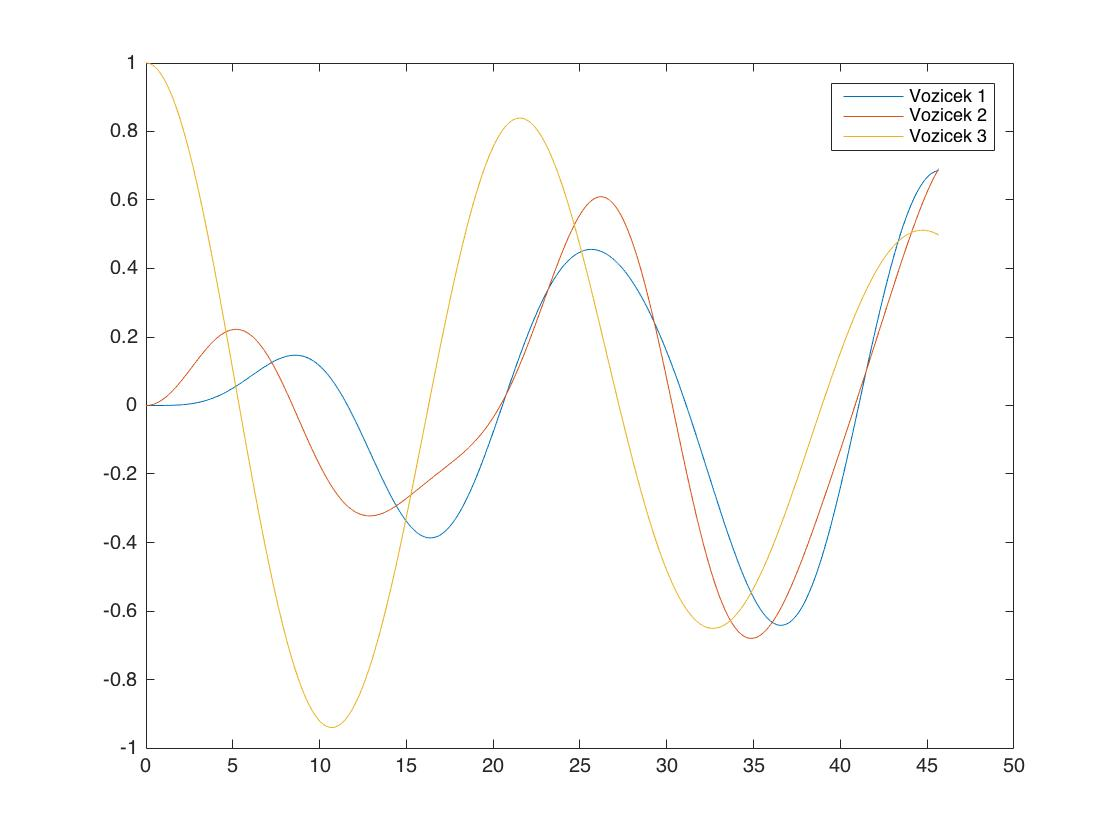
\includegraphics[width=0.80\textwidth]{vozicki.jpg}
\end{figure}
 
\section{Množenje v smereh}
V datotekah \emph{zmnozi.m} in \emph{determinanta.m} se nahajata funkciji, kot sta podanai v navodilih naloge. V datoteki \emph{aliSmoEnaki.m} se nahaja funkcija, ki preveri, če vhodni vektor kakšno spremenljivko podvojeno. Funkcija \emph{predznakPermutacije.m} vrne predznak permutacije, ki ga potrebujemo za izračun determinante. V datoteki \emph{test.m} se nahaja algoritem, ki nadomešča $n$ for zank, ki smo ga dobili na \cite{vir1}. V spremenljivki $start\_ranges$ so shranjeni začetni indeksi for zank,  v spremenljivki $end\_ranges$ pa so shranjene končne vrednosti for zank. Vse te datoteke uporabimo v \emph{zmnoziEksperiment}, kjer implementiramo množenje tenzorja poljubnih dimenzij v neki smeri,ter v \emph{determinantaEksperiment}, kjer s pomočjo tenzorjev lahko izračunamo determinanto za kvadratno matriko poljubne velikosti. Težava računanja determinante na tak način se pojavi že pri matrikah nizkega ranga, saj postane tezor $X$ prevcej velik v prostorskem smislu. 

Sedaj še razložimo, kako smo prišli do tenzorja $X$. 
Iščemo tak $X\in \R^{3\times3\times3}$, da bo za matriko $A \in R^{3\times 3}$ veljalo:
\begin{align}
\label{determinanta}
	\det(A) = X \times_1 a_1^T \times_2 a_2^T \times_3 a_3^T
\end{align}
Ker je $X \times_1 a_1^T \times_2 a_2^T \times_3 a_3^T \in \R^{1\times1\times1}$, ga lahko smatramo kot skalar. Posledično velja formula: 
\begin{align*}
	X \times_1 a_1^T \times_2 a_2^T \times_3 a_1^T = (a_3^T\otimes a_2^T\otimes a_3^T)\ve(X)
\end{align*}
Od tu je jasno, da če želimo, da velja formula \eqref{determinanta}, mora veljati:
\begin{align*}
	X_{ijk} = \begin{cases}
	1 , &(i j k) ~\text{je soda permutacija}  \\
	-1, &(i j k) ~\text{je liha permutacija}  \\
	0, &sicer\\
	\end{cases}
\end{align*}
Na idejno enak način lahko $X$ posplošimo na poljubne velikosti tako, da ga lahko uporabimo za izračun determinante matrik višjih dimenzij., kar smo uporabili v datoteki \emph{determinantaEksperiment}.  


\section{HOSVD}
Pri tej nalogi smo najprej implementirali \emph{razpri.m}, ki nam tenzor razpre v $i$-ti izbrani smeri.  Druga nova datoteka pri tej nalogi pa je \emph{hosvd.m}, ki za vhodne parametre sprejeme trorazsežen tenzor $T$, ter željene dimenzije njegovega jedra. Funkcija nam vrne jedro, ter matrike $U_i$ z ortonormiranimi stolpci. Z mojo implementacijo metoda \emph{hosvd.m} porabi preveč spomina, zato sem namesto $\rand(5, 200, 200)$ vzel $\rand(5, 100, 100)$, da še vseeno dobim nek rezultat. Spodaj je prikazano jedro $G$, ki ga dobimo kot aproksimacijo v $\R^{3 \times 3 \times 3}$. 

\begin{align*}
G(:, :, 1) &= 
\begin{pmatrix}
-112.2054&0.00086499&-0.033207\\
0.067136&-0.31259&-0.48249\\
-0.13896&0.42642&-0.24045\\
\end{pmatrix}\\
G(:, :, 2) &= 
\begin{pmatrix}
-0.015684&-0.91549&0.59074\\
-0.13908&0.52085&0.061513\\
0.29164&-0.21774&-0.40183\\
\end{pmatrix}\\
G(:, :, 3) &= 
\begin{pmatrix}
0.021486&0.62483&1.6935\\
0.47255&0.16888&-0.6975\\
-0.31551&-0.55424&0.42156\\
\end{pmatrix}
\end{align*}



\begin{thebibliography}{1}
	\bibitem{vir1}
	https://stackoverflow.com/questions/7186518/function-with-varying-number-of-for-loops-python
	\bibitem{vir2}
	https://www.fmf.uni-lj.si/$\sim$plestenjak/Vaje/Primeri.htm
\end{thebibliography}









\end{document}